\subsection{Сферическая тригонометрия}
\label{sec:spher-trig}
\begin{wrapfigure}[10]{r}{.3\tw}
	\centering
	\vspace{-1pc}
	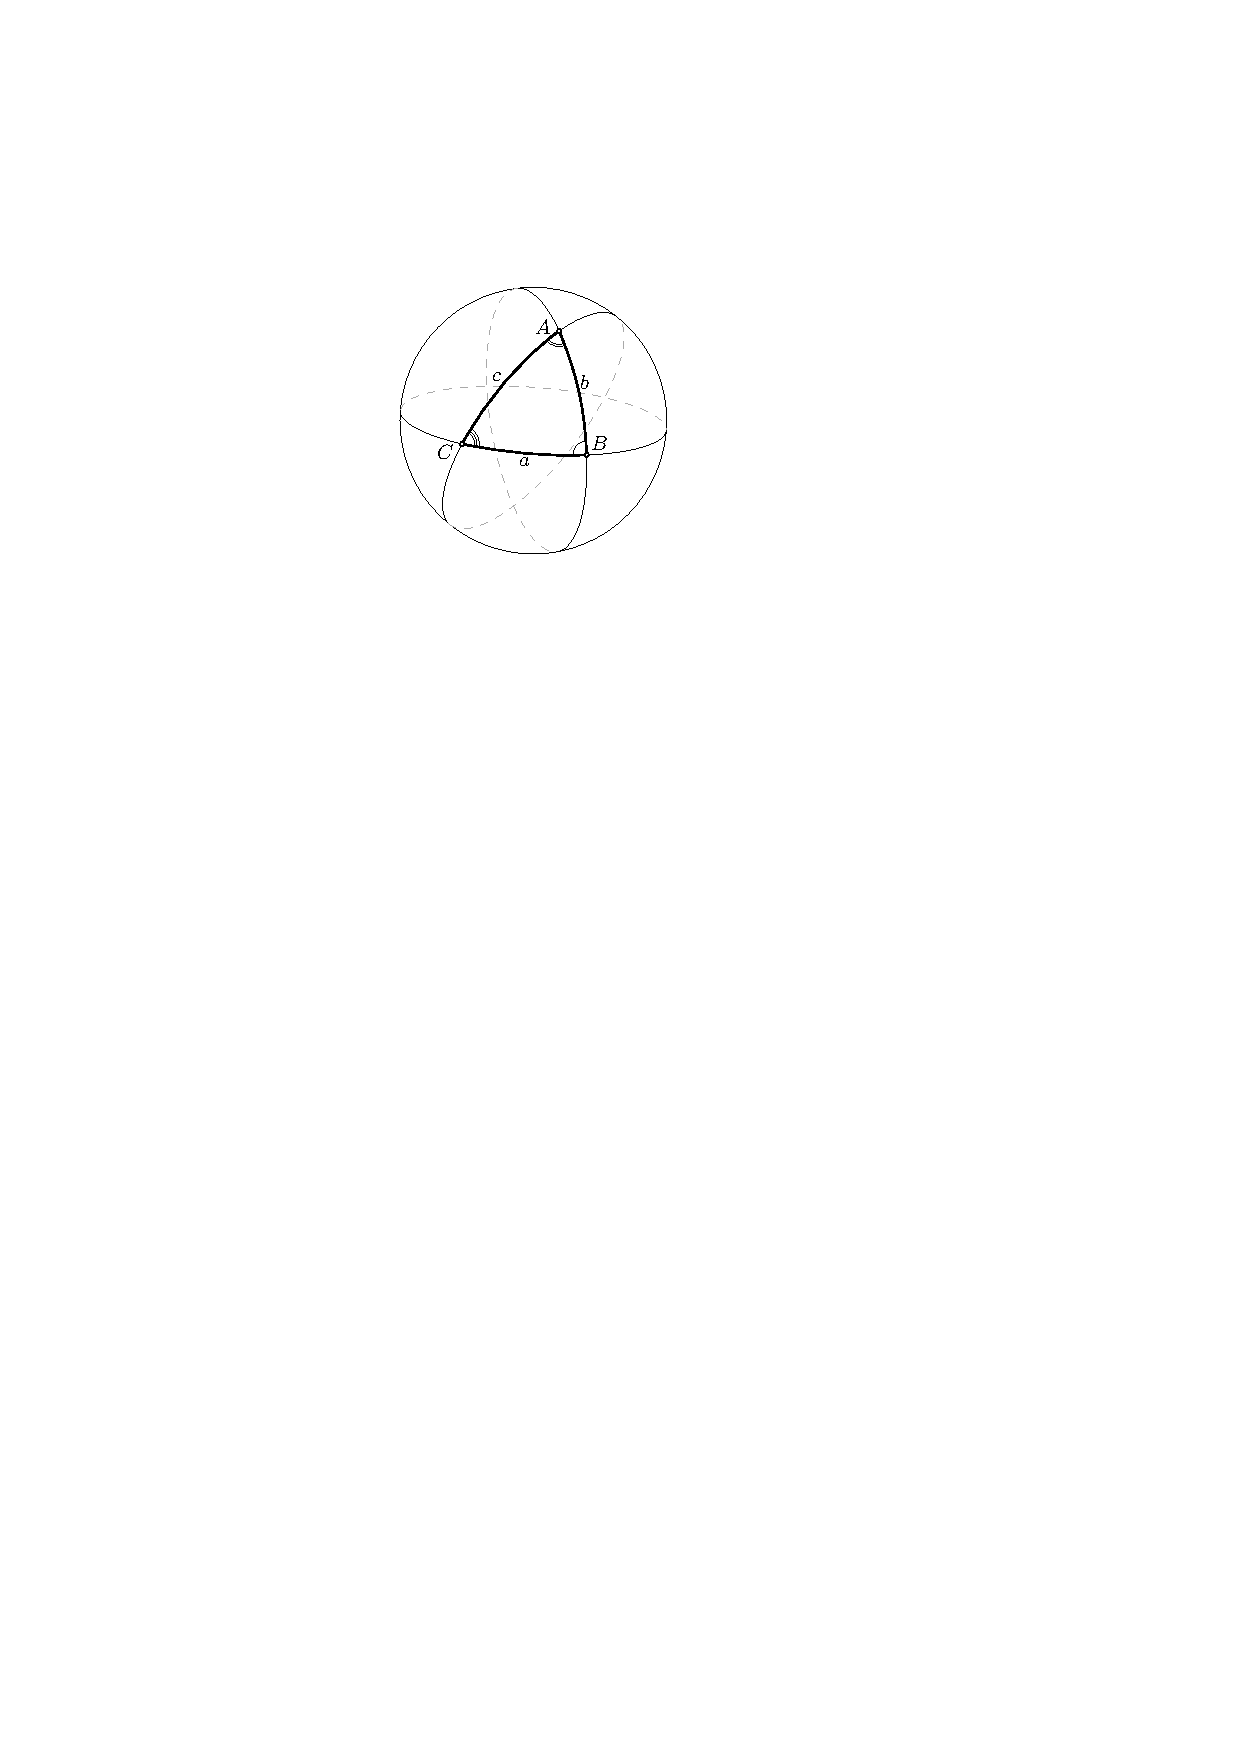
\includegraphics[width=0.3\textwidth]{spher-trigonom}
	\caption{Сферический треугольник}
\end{wrapfigure}
Для решения некоторых задач астрономии, связанных с видимыми положениями небесных тел, требуются знания о сферической тригонометрии. \imp{Сферический треугольник}~--- фигура на поверхности сферы, состоящая из трёх точек и трёх дуг больших кругов, соединяющих эти точки. Пусть $A$, $B$ и $C$~--- углы сферического треугольника, а $a$, $b$ и $c$~--- его стороны.

Сферические треугольники обладают следующими свойствами:
\begin{enumerate}
	\item Два сферических треугольника равны, если они подобны.
	\item Каждая сторона меньше суммы двух других сторон и больше их разности.
	\item Сумма всех сторон $a+b+c$ всегда меньше $2\pi$.
	\item Сумма углов сферического треугольника $\pi < A + B + C < 3\pi$.
	\item Разность суммы двух углов и третьего угла меньше $\pi$
\end{enumerate}

Площадь сферического треугольника определяется по формуле:
\begin{equation}
	S = R^2( A + B + C - \pi),
\end{equation}
где $A + B + C - \pi$~--- \imp{сферический избыток}.

Рассмотрим сферический треугольник $ABC$, радиус векторы вершин соответственно $\vec{a}$, $\vec{b}$ и $\vec{c}$. причем из определения сферы $|\vec{a}| = |\vec{b}| = |\vec{c}| = r$. Пусть против вершин $A$, $B$ и $C$ лежат стороны с угловой мерой $a$, $b$ и $c$ соответсвенно. Повернем сферические координаты и нормируем так, чтобы $\vec{a} = (0, 0, 1)$, $\vec{b} = (\sin c, 0, \cos c)$, тогда $ \vec{c} = (\sin b \cos A, \sin b \sin A, \cos b)$.

Теперь запишем выражение для $\scalar{b}{c}$:
\begin{equation}
	\scalar{b}{c} = \cos a = \sin c \sin b \cos A + \cos c \cos b.
	\label{eq:spher-astro-cos-1}
\end{equation}
Аналогично,
\begin{gather}
	\scalar{a}{c} = \cos b = \sin a \sin c \cos B +  \cos a \cos c,\\
	\scalar{a}{b} = \cos c = \sin a \sin b \cos C + \cos a \cos b.
	\label{eq:spher-astro-cos-1-1}
\end{gather}
Выразим отсюда $\cos A$:
\begin{equation}
	\cos A = \frac{\cos a - \cos c \cos b}{\sin c \sin b}.
	\label{eq:spher-astro-cos-2}
\end{equation}
Формулы \eqref{eq:spher-astro-cos-1}\,--\,\eqref{eq:spher-astro-cos-2} называются \term{сферической теоремой косинусов} \imp{для стороны} \eqref{eq:spher-astro-cos-1}\,--\,\eqref{eq:spher-astro-cos-1-1} и, соответственно \imp{для угла} \eqref{eq:spher-astro-cos-2}.

Из основного тригонометрического тождества имеем:
\begin{multline*}
	\sin^2 A = 1 - \cos^2 A = 1 - \left[ \frac{\cos a - \cos c \cos b}{\sin c \sin b} \right]^2 = \\
	= \frac{\sin^2 c \sin^2 b - \cos^2 a + 2\cos a \cos c \cos b - \cos^2 c \cos^2 b}{\sin^2 c \sin^2 b}=\\
	= \frac{(1 - \cos^2 c)(1 -  \cos^2 b) - \cos^2 a + 2\cos a \cos c \cos b - \cos^2 c \cos^2 b}{\sin^2 c \sin^2 b}=\\
	= \frac{1 - \cos^2 c - \cos^2 b + \cos^2 c \cos^2 b -\cos^2 a}{\sin^2 c \sin^2 b} + \\
	+ \frac{2\cos a \cos c \cos b - \cos^2 c \cos^2 b}{\sin^2 c \sin^2 b} = \\
	= \frac{1 - \cos^2 c - \cos^2 b - \cos^2 a + 2\cos a \cos c \cos b}{\sin^2 c \sin^2 b}.
\end{multline*}
Извлекая квадратный корень из левой и правой части и деля их на $\sin a$ имеем
\begin{equation*}
	\frac{\sin{A}}{\sin a} = \frac{\sqrt{1 - \cos^2 c - \cos^2 b - \cos^2 a + 2\cos a \cos c \cos b}}{\sin a \sin b \sin c}.
\end{equation*}
Заметим, что правая часть равенства циклична по переменным $a$, $b$ и $c$, следовательно, \term{сферическая теорема синусов} имеет вид
\begin{equation}
	\frac{\sin A}{\sin a} = \frac{\sin B}{\sin b} = \frac{\sin C}{\sin c}.
\end{equation}

Напоследок получим \term{формулу пяти элементов}. Для этого запишем теорему косинусов в выразим в ней один из косинусов, применяя ее же:
\begin{gather}
	\cos a = \sin c \sin b \cos A + \cos c \cos b,\nonumber\\
	\cos a = \sin c \sin b \cos A + \left( \sin a \sin b \cos C + \cos a \cos b \right)\cos b,\nonumber\\
	\cos a - \cos a \cos^2 b = \sin c \sin b \cos A + \sin a \sin b \cos b \cos C,\nonumber\\
	\cos a \sin^2 b = \sin c \sin b \cos A + \sin a \sin b \cos b \cos C,\nonumber\\
	\cos a \sin b = \sin a \cos b \cos C + \sin c \cos A.
\end{gather}

\term{Параллактический треугольник}~--- треугольник на небесной  сфере, образованный пересечением небесного меридиана, вертикального круга и часового круга светила. \imp{Вертикальный круг}~--- большой круг небесной сферы, проходящий через надир, зенит и светило. \imp{Часовой круг}~--- большой круг небесной сферы, проходящий через полюса мира и наблюдаемое светило.

Применяя теоремы синусов и косинусов к параллактическому треугольнику, нетрудно получить следующие соотношения:
\begin{gather}
	\cos z=\sin\varphi\sin\delta+\cos\varphi\cos\delta\cos t\\
	\sin z\sin A=\cos\delta\sin t\\
	\sin z\cos A=-\cos\varphi\sin\delta+\sin\varphi\cos\delta\cos t
\end{gather}

Напоследок, используя сферическую теорему косинусов, получим \term{уравнение большого круга}. Пусть на сфере заданы сферические координаты $(\lambda, \varphi)$, где $\lambda$~--- угол проекции вектора на плоскость $Oxy$ с осью $Ox$, см.~Раздел\;\ref{sec:coord-systems}, а $\varphi$~--- угол между вектором в плоскостью $Oxy$. Найдем уравнение большого круга с наклонением $i$, восходящий узел которого находится в точке $(\lambda_0, 0)$. 

Для этого рассмотрим произвольную точку $(\lambda, \phi)$ на этом большом круге и один из его полюсов $(\lambda - 90^\circ, 90^\circ - i)$. По определению большого круга каждая его точка отстоит от полюса на $90^\circ$. Запишем сферическую теорему косинусов для треугольника полюс системы координат -- полюс большого круга -- произвольная точка на большом круге:
\begin{gather}
    \cos 90^\circ = \cos i \cos (90 - \varphi) + \sin i \sin (90 - \varphi) \cos (\lambda - (\lambda_0 - 90^\circ)),\nonumber \\
    0 = \cos i \sin \varphi - \sin i \cos \varphi \sin (\lambda - \lambda_0),\nonumber\\
    \boxed{\frac{\tg \varphi}{\tg i} = \sin (\lambda - \lambda_0),}
    \label{eq:great-circle-eq}
\end{gather}
полученное уравнение является \imp{уравнением большого круга}.